% !TEX root = ../../report.tex

\section{Recommendation methods}

This section aims to describe the algorithms and methods which we have developed or borrowed from others which will be included in our experiments.

\marginpar{TODO: Motivate the explanation of the methods}
One could imagine to final system to leverage multiple recommendation techniques. When users are new to the system they
are recommended the most popular items, until enough data is collected to provide personalized recommendations. Another solution would be to use pre-computed item similarities and recommend similar items to the item currently being viewed by the user. We also wish to use these methods as benchmarks.


\subsection{Recommender algorithms}

The section will describe the different recommendation algorithms included in our experiments.

\subsubsection{Most-popular Recommender}

We developed a simple most-popular recommender that uses result dithering to \emph{randomize} the recommendations to the users. One could imagine multiple categories of most popular recommendations: Most wanted, most purchased or a combination. Dithering adds \emph{noise} to the algorithm, which permutes the results in such a way that the top few results have a high probability of remaining on the top spots, but as one goes deeper into the results, the degree of mixing increases dramatically. It is important to note that dithering is \emph{guaranteed} to make off-line performance worse, but is likely to make the actual performance better as the user is not presented with the same list of recommendations every time. We have experimented with two different methods of dithering:


\begin{itemize}
\item $Score = log_2(rank+x) - runif(y, z)$
\item $Score = log_2(rank+x) - y*rexp(z)$
\end{itemize}

The $runif$ function draw samples from a uniform distribution where $y$ specifies the lower boundary of the output interval and $z$ specifies the upper boundary. The probability density function of the uniform distribution is $P(x) = \frac{1}{z-y}$ anywhere within the interval $[y, z)$, and zero elsewhere. The $rexp$ function draws a random number from an exponential distribution, where $z$ specifies the $\lambda$ value, which is set to $\frac{1}{z}$. Figure \ref{fig:expdist} shows the exponential probability density function given different $\lambda$ values.

% Vertical alignment of equation and plot.
\begin{figure}[H]
\label{fig:expdist}
  \centering
    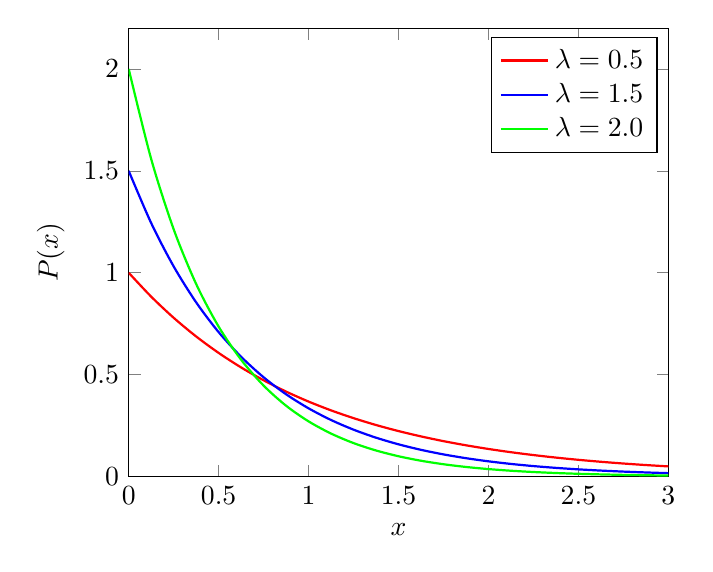
\begin{tikzpicture}
      \begin{axis}[
      	xlabel={$x$},
      	ylabel={$P(x)$},
      	ymin = 0, ymax=2.2, xmin=0, xmax=3,
      	legend entries={$\lambda=0.5$,$\lambda=1.5$,$\lambda=2.0$},
      	domain=0:3,
      ]
      \addplot[thick,smooth,red]{exp(-x)};
      \addplot[thick,smooth,blue]{1.5*exp(-1.5*x)};
      \addplot[thick,smooth,green]{2.0*exp(-2.0*x)};
      \end{axis}
    \end{tikzpicture}
    \caption{Probability density function, exponential distribution}
\end{figure}

Given $x=5$, $y=0$ and $z=6$ using the uniform distribution we get the following permutations of the original ranking in 10 runs:

%http://tex.stackexchange.com/questions/131595/plot-with-min-max-bar-and-two-average-points

\begin{table}[H]
	\centering
	\begin{tabular}{*{11}l}
	\toprule
	\multicolumn{1}{l}{\#Run} & \multicolumn{10}{l}{Result} \\ \midrule
	1 	& 8 & 3 &  24 &  20 &  1 &  19 &  22 &  15 &  42 &  36 \\
	2 	& 2 &  0 &  1 &  32 &  20 &  3 &  35 &  34 &  43 &  10 \\
	3	& 7 &  1 &  3 &  12 &  2 &  25 &  0 &  9 &  24 &  27\\
	4	& 0 &  4 &  3 &  5 &  7 &  16 &  26 &  22 &  13 &  33\\
	5	& 0 &  10 &  8 &  1 &  15 &  5 &  30 &  17 &  11 &  35\\
	6	& 7 &  4 &  6 &  12 &  2 &  1 &  19 &  0 &  27 &  9\\
	7	& 1 &  5 &  0 &  2 &  9 &  3 &  20 &  12 &  4 &  31\\
	8	& 0 &  1 &  2 &  5 &  39 &  4 &  15 &  41 &  10 &  22\\
	9	& 4 &  6 &  0 &  3 &  1 &  29 &  36 &  31 &  35 &  20\\
	10	& 5 &  1 &  0 &  8 &  3 &  18 &  25 & 24 & 2 & 28\\
	\bottomrule
\end{tabular}
\end{table}

Given $x=1$, $y=3.0$ and $z=2.5$ using the exponential distribution we get the following permutations of the original ranking in 10 runs:

\begin{table}[H]
	\centering
	\begin{tabular}{*{11}l}
	\toprule
	\multicolumn{1}{l}{\#Run} & \multicolumn{10}{l}{Result} \\ \midrule
	1	& 2 &  4 &  0 &  35 &  3 &  1 &  15 &  72 &  9 &  5\\
	2	& 0 &  10 &  11 &  17 &  1 &  3 &  8 &  41 &  15 &  5\\
	3	& 44 &  1 &  0 &  15 &  9 &  4 &  5 &  59 &  26 &  2\\
	4	& 0 &  98 &  1 &  4 &  2 &  41 &  8 &  26 &  11 &  94\\
	5	& 0 &  6 &  1 &  2 &  70 &  4 &  19 &  14 &  8 &  3\\
	6	& 2 &  5 &  0 &  16 &  15 &  18 &  1 &  3 &  32 &  6\\
	7	& 2 &  65 &  4 &  0 &  3 &  45 &  8 &  1 &  48 &  36\\
	8	& 3 &  49 &  5 &  0 &  2 &  82 &  8 &  77 &  11 &  4\\
	9	& 0 &  1 &  21 &  8 &  4 &  85 &  2 &  6 &  47 &  3\\
	10	& 0 &  1 &  21 &  70 &  11 &  20 &  2 & 10 & 9& 3 \\
	\bottomrule
\end{tabular}
\end{table}

where 0 is the most popular item before the permutation. The results show that alternative two has a larger occurrence of items that are further down in the list. This is due to the fact that the exponential distribution can output large values, in theory up to infinity, with a decreasing probability. The values of $x$, $y$ and $z$ can be modified to achieve the desired degree of mixing.

\subsubsection{Item-Average}

Item average is a simple recommender that always estimates the preference for an item to be the average of all known preference values for that item. No information about the individual users is taken into account. This recommender can therefore be considered a \emph{highest rated} recommender, as it is likely to recommend the highest rated items. The following equation shows the rating prediction procedure:

\begin{equation}
\label{equation:itemaverageratingprediction}
u(c,s) = k * \sum_{c' \epsilon C} u(c',s)
\end{equation}

where $k$ is a normalization factor ($1/|C|$). This is very similar to collaborative filtering, except for the fact that the user similarity $sim(c, c')$ has been taken out of the equation. This is the same as saying that all user similarities are the same. It is also worth mentioning that this method is not suited for binary ratings, as the result is likely to be highly random, and should therefore not be used without item ratings to average.

\subsubsection{User-based Collaborative Filtering}

Recommend items by finding similar users. This is often harder to scale because of the dynamic nature of users. The pearson correlation coefficient is used to calculate the user similarities. For a more in depth description of user-based collaborative filtering see Section \ref{subsec:cf}.

\subsubsection{Item-based Collaborative Filtering}

Calculate similarity between items and make recommendations. Items usually don't change much, so this often can be computed offline. For a more in depth description of item-based collaborative filtering see Section \ref{subsec:cf}.%

\subsubsection{ALS-WR}

%ALS-WR only? matrix factorization method which can be combined with our implicit ratings

Alternating-least-squares with weighted-$\lambda$-regularization (ALS-WR) was designed fro the Netflix Prize Competition \cite{Netflix}, where it obtained an RMSE score of 0.8975, which was one of the best results based on a pure method.
in theory up to infinity
Alternating-least-squares is a method to solve Equation \ref{equation:minimize}. Since both $q_{s}$ and $p_{c}$ are unknown, the equation is not convex. However if we fix one of the unknowns, the optimization problem becomes quadratic and can be solved optimally. The ALS technique rotate between fixing the $q_{s}$'s and fixing the $p_{c}$'s. When all the $p_{c}$'s are fixed, the system recomputes the $q_{s}$'s by solving a least-squares problem, and vica versa. This ensures that each step decreases the error until convergence. What makes ALS favorable over the simpler and faster stochastic gradient descent is two things. ALS can be parallelized since the system computes the $q_{s}$'s independently of the other item factors, the same can also be applied to the user factors. The second case if for systems centered around implicit data. Because the training set cannot be considered sparse, looping over each single training case as gradient descent would not be practical, but ALS can efficiently handle such cases \cite{Hu2008}.\newline

ALS solves the low-rank matrix factorization as follows:

\begin{itemize}
\item Step 1: Initialize the matrix M by assigning the average rating for that movie as the first row, and a small random numbers for the remaining entries;
\item Step 2: Fix P, solve Q by minimizing the objective function (the sum of squared errors);
\item Step 3: Fix Q, solve by minimizing the objective function similarly;
\item Step 4: Repeat Steps 2 and 3 until a stopping criterion is satisfied.
\end{itemize}

Zhou et. al. \cite{Zhou2008} used the difference in RMSEs between the rounds as a stopping criterion. Without regularization ALS might lead to overfitting due to the many free parameters. Regularization was therefore introduced in the form of weighted-$\lambda$-regularization to prevent the model from overfitting.

\begin{equation}
f(P, Q) = \sum_{(c,s)\epsilon C} (u(c,s) - p^{T}_{c}q_{s})^{2} + \lambda (\sum_{c} n_{p_{c}} \Vert p_{c} \Vert ^{2} + \sum_{s} n_{q_{s}} \Vert q_{s} \Vert ^{2})
\label{WeightedLamba}
\end{equation}

where $n_{p_{c}}$ and $n_{q_{s}}$ denote the number of ratings of user $c$ and item $s$ respectively. $S_{c}$ denote the set of items $s$ that user $c$ rated, then $n_{p_{c}}$ is the cardinality of $S_{c}$; similarly $C_{s}$ denotes the set of users who rated item $s$, and $n_{q_{s}}$ is the cardinality of $I_{s}$. A given column of P, $p_{c}$ is found by solving a regularized linear least squares problem involving the known ratings of user $c$, and the feature vectors $q_{s}$ of the items that user $c$ has rated. Similarly, we can compute individual $q_{s}$'s via a regularized linear least squares solution, using the feature vectors of users who rated item $j$, and their ratings of it.

%Description of implicit extension of ALS-WR

\subsubsection{Content-based}

\marginpar{TODO: Complete motivation}
As previously mentioned content-based recommendation does not suffer as much from the cold-start problem as
collaborative filtering approaches. 

To build features for content-based recommendations we examined the content in the product database. To find the product-type, material, style and color we analyzed the content of the title, description and meta-description fields extracting the most used keywords after removing the stopwords, which we combined and grouped for the different attributes. Since product descriptions could be either in Norwegian or in English we had to include the words from both languages. We also experimented with stemming from the nltk software package in python, but since it did not improve our results it was not used in the final implementation. E.g. to determine if a product-type falls under the \emph{sweater} category we check for the following keywords: \emph{sweater, cardigan, jumper, hoody ,genser and genseren}. We attempt to extract the following features from the product-database content:


\begin{itemize}
\item Price: Grouped into price brackets
\item Brand/Storename
\item Category: E.g. dress, jacket, top, pants and boots
\item Material: E.g. Cotton, wool, polyester, leather
\item Style: E.g. Classic, Modern, Comfy, Sexy
\item Color
\end{itemize}

It was a pleasant surprise to find out that 5,060 out of 5,855 items could be found in the
product database and be assigned features. The following table shows an overview over how many items we were able to extract the different features for.

\begin{table}[H]
	\centering
	\begin{tabular}{l l}
	\toprule
	Attribute & Percentage  \\ \midrule
	Price 			& 1.000 \\ 
	Brand 			& 0.742 \\ 
	Category 		& 0.628 \\ 
	Material 		& 0.408 \\ 
	Style 			& 0.314 \\ 
	Color 			& 0.162
	\\ \bottomrule
	\end{tabular}
\end{table}

Price, brand and product-type can be found for \emph{most} items, while material style and color could only be found for a minority of the items. The dataset is in no way ideal for content-based recommendation as it highlights on of the main weakness of content-based methods, namely that they require rich descriptions of items to build well informed user profiles. As mentioned in \cite{meyer2012recommender} this is most often not the case in real applications. 

\marginpar{Mention what item-based methods will be used}

\subsection{Cold-start Solutions}

Due to limitations, mainly in the form of lacking data the number of cold-start solutions
we are currently able to experiment with is fairly limited. As we never got access to
user-data, we have to cross out RBLF and other methods requiring user features. This leaves us with
Naive Filterbots \cite{Park2006} which easily could be combined with our implicit ratings.

\subsubsection{Filterbots}

The main reasons for experimenting with filterbots is simplicity, the fact that it easily could
be combined with our implicit ratings in addition to the fact that previous experiments \cite{Agarwal2009, Agarwal2010} show that its performance is close to the state-of-the-art methods. It is worth to keep in mind that filterbots was developed for traditional collaborative filtering methods and it will be interesting to see how the filterbots affect the performance of ALS-WR. Filterbots can potentially help solve the cold-start user problem by making it possible for new users to connect to users that capture the general underlying trends of the entire user group. Filterbots are mainly meant to improve performance when data is scarce and not to degrade performance when data is plentiful.

Similarly as in \cite{Park2006} we decided to experiment with global bots. We have currently implemented the following bots:
A \emph{BrandBot} which rates an item based on the brands average rating, an \emph{AverageBot} which rates an item based on their average rating given to it, a \emph{CriticBot} which selects $n$ critics among the most active users and rate items based on their average rating, a \emph{PopularityBot} which rates an item based on its popularity, more ratings equals a higher rating. A filterbot takes the training set as input and generates a set of ratings which are then added to the training set. Both the \emph{AverageBot} and \emph{BrandBot} can be seen to incorporate the implicit rating factors such as recency into the ratings generated. However, for the \emph{PopularityBot} and \emph{Critic} but we wish to implement additional functionality to ensure that the new users are connected with items that are relevant right now and not consider outdated items or users which are no longer active. Since we have access to timestamps we could e.g. make the \emph{PopularityBot} rate items based on their popularity the last couple of weeks instead of over the entire dataset period. Similarly, critics can be selected based on their activity the couple of weeks/months.

\marginpar{TODO: Describe implementation?}

